% ==============================================================================
% 插曲 1：初学学生语言 (Intermezzo 1: Beginning Student Language)
% ==============================================================================

\intermezzo{插曲 1：初学学生语言 (BSL)}
\label{sec:intermezzo01}

在本书的第一部分中，我们通过直观的示例与非正式的说明学习了初学学生语言（BSL）。现在是时候停下匆忙的脚步，系统性地审视这门小巧却极其严谨的编程语言的全貌了。

一门程序设计语言由两个核心部分构成：
\begin{itemize}
  \item \term{句法}（Syntax）：规定了哪些符号序列构成合法的程序句子（包括词汇与文法）；
  \item \term{语义}（Semantics）：精确阐明了合法的程序句子在计算机内部如何一步步执行归约（计算含义）。
\end{itemize}

本插曲将带你全面梳理 BSL 的词汇表、核心文法、等量代换计算模型、短路布尔求值、结构体运行机制以及详尽的常见错误诊断手册。

% ==============================================================================
\intermezzosection{BSL 词汇 (BSL Vocabulary)}
\label{sec:int01_vocabulary}
% ==============================================================================

在任何语言中，基本词汇被称为\term{词素}或\term{词法记号}（Tokens）。BSL 的核心词汇包含四类：
\begin{enumerate}
  \item \textbf{字面常量}（Literal Constants）：数（如 \code{42}, \code{3.14}, \code{-5/9}）、布尔值（\code{\#true}, \code{\#false}）、字符串（如 \code{"hello"}）以及图像；
  \item \textbf{标识符}（Identifiers / Names）：变量名、函数名与字段名。BSL 对标识符的命名极其宽容，几乎允许任何不包含空格和圆括号的字符序列（例如 \code{string->number}, \code{distance-to-0}, \code{traffic-light?} 等）；
  \item \textbf{关键字}（Keywords）：具有特殊语法地位的保留字，如 \code{define}, \code{define-struct}, \code{cond}, \code{else}, \code{check-expect} 等；
  \item \textbf{标点符号}：开闭圆括号 \code{(} 与 \code{)}，以及等价的开闭方括号 \code{[} 与 \code{]}。
\end{enumerate}

\begin{figure}[htbp]
  \centering
  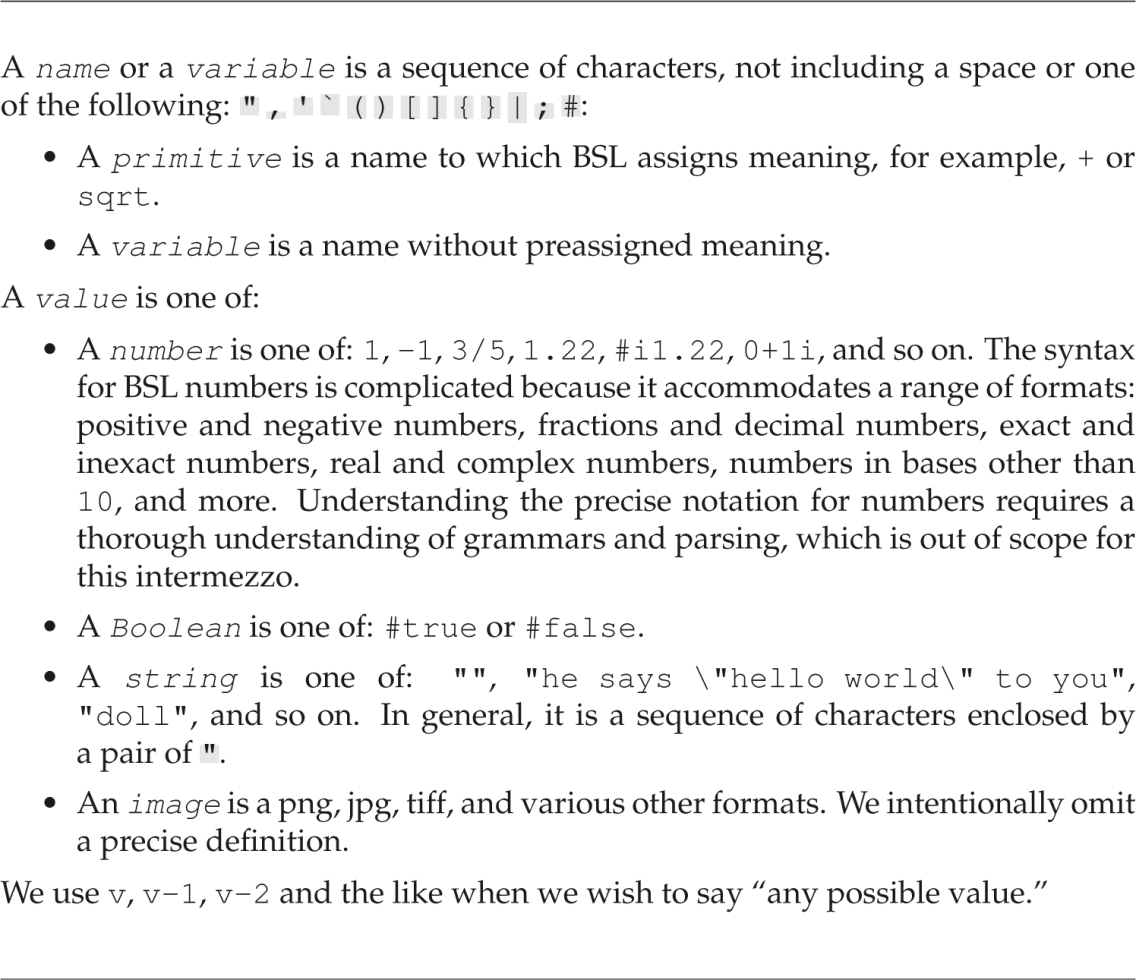
\includegraphics[width=0.85\textwidth]{images/00134.png}
  \caption{BSL 核心词汇体系}
  \label{fig:bsl_vocab}
\end{figure}

% ==============================================================================
\intermezzosection{BSL 文法 (BSL Grammar)}
\label{sec:int01_grammar}
% ==============================================================================

文法规定了如何将词汇组合为合法的表达式与定义。计算机科学家使用一种称为“上下文无关文法”（Context-Free Grammar）的代数表示法来定义语言规则。

\begin{figure}[htbp]
  \centering
  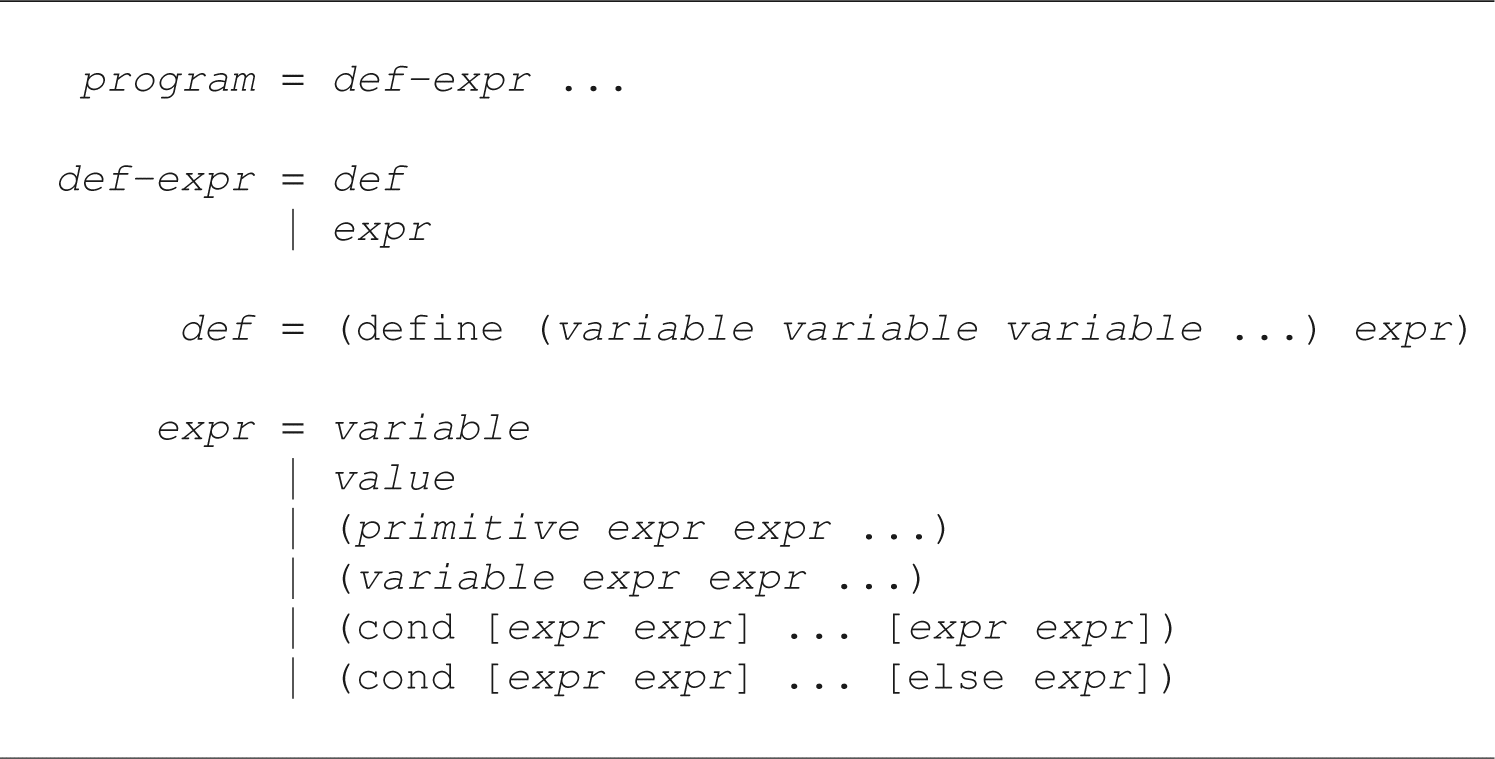
\includegraphics[width=0.85\textwidth]{images/00135.png}
  \caption{BSL 核心表达式与定义文法}
  \label{fig:bsl_grammar}
\end{figure}

图~\ref{fig:bsl_grammar} 展示了 BSL 的核心文法法则：
\begin{itemize}
  \item 一个\term{程序}（Program）是由零个或多个定义和表达式构成的序列；
  \item 一个\term{定义}（Definition）具有以下形式之一：
    \begin{itemize}
      \item 常量定义：\code{(define } Variable \code{ } Expression\code{)}
      \item 函数定义：\code{(define (} FunctionName Variable $\dots$ Variable\code{) } Expression\code{)}
      \item 结构体类型定义：\code{(define-struct } StructureName \code{[} FieldName $\dots$ FieldName\code{])}
    \end{itemize}
  \item 一个\term{表达式}（Expression）可以是值、变量、函数应用、条件表达式或逻辑运算。
\end{itemize}

\begin{figure}[htbp]
  \centering
  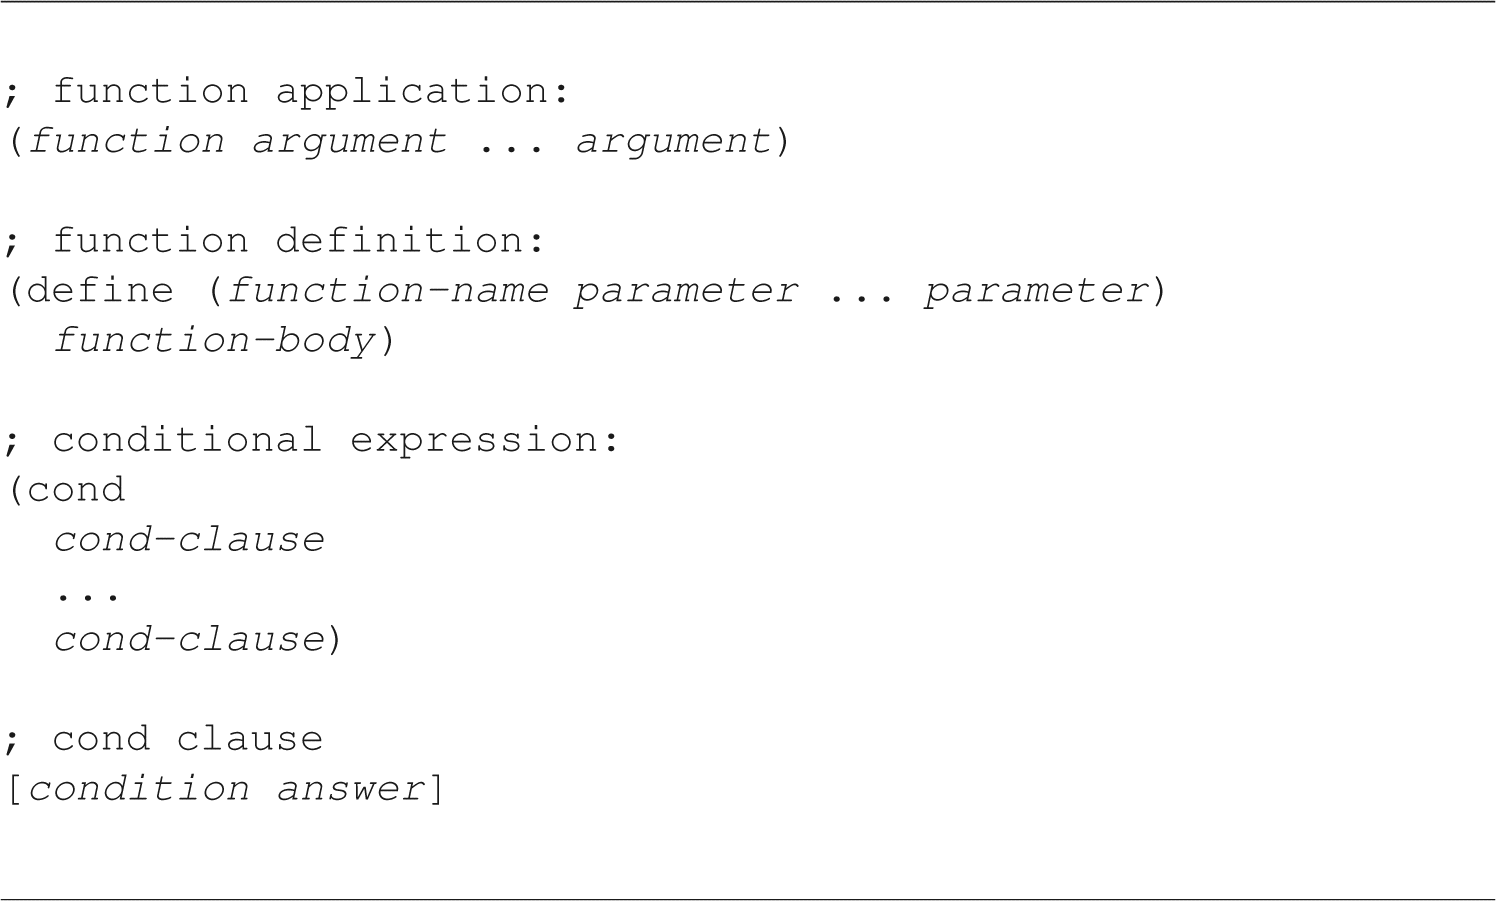
\includegraphics[width=0.75\textwidth]{images/00136.png}
  \caption{BSL 句法命名规范与元变量说明}
  \label{fig:bsl_naming_conventions}
\end{figure}

\begin{exercise}{文法合法性辨析 1}{116}
根据图~\ref{fig:bsl_grammar} 的文法规则，判断以下句子是否为合法的 BSL 表达式：
\begin{lstlisting}[language=BSL]
x
(= x 5)
(= (= x 5) 0)
\end{lstlisting}
\end{exercise}

\begin{exercise}{文法合法性辨析 2}{117}
判断以下语句是否为合法的 BSL 定义或表达式：
\begin{lstlisting}[language=BSL]
(3 + 4)
number?
(x)
\end{lstlisting}
\end{exercise}

\begin{exercise}{文法合法性辨析 3}{118}
仔细观察以下句子，解释为什么它们是合法或非法的：
\begin{lstlisting}[language=BSL]
(define (f x) x)
(define (f x) y)
(define (f x y) 3)
\end{lstlisting}
\end{exercise}

\begin{exercise}{文法合法性辨析 4}{119}
判断以下句子是否符合 BSL 文法：
\begin{lstlisting}[language=BSL]
(define (f) 10)
(define (f x y z) (x))
(define (f) (cond [(> 1 0) 10] [else 20]))
\end{lstlisting}
\end{exercise}

\begin{exercise}{综合文法甄别}{120}
区分以下句子中哪些是合法的 BSL 结构，哪些是非法的：
\begin{lstlisting}[language=BSL]
(+ 1 (not x))
(+ 1 2 3)
(cond)
(cond [else 10])
(cond [(< x 0) 10] [else 20])
\end{lstlisting}
\end{exercise}

% ==============================================================================
\intermezzosection{BSL 语义 (BSL Meaning)}
\label{sec:int01_meaning}
% ==============================================================================

如果一个程序在文法上是合法的，它就拥有了明确的\term{计算语义}。BSL 的最迷人之处在于：\textbf{它的语义完全可以用初等代数中的“等量代换”（Replacing Equals by Equals）来解释！}

\begin{figure}[htbp]
  \centering
  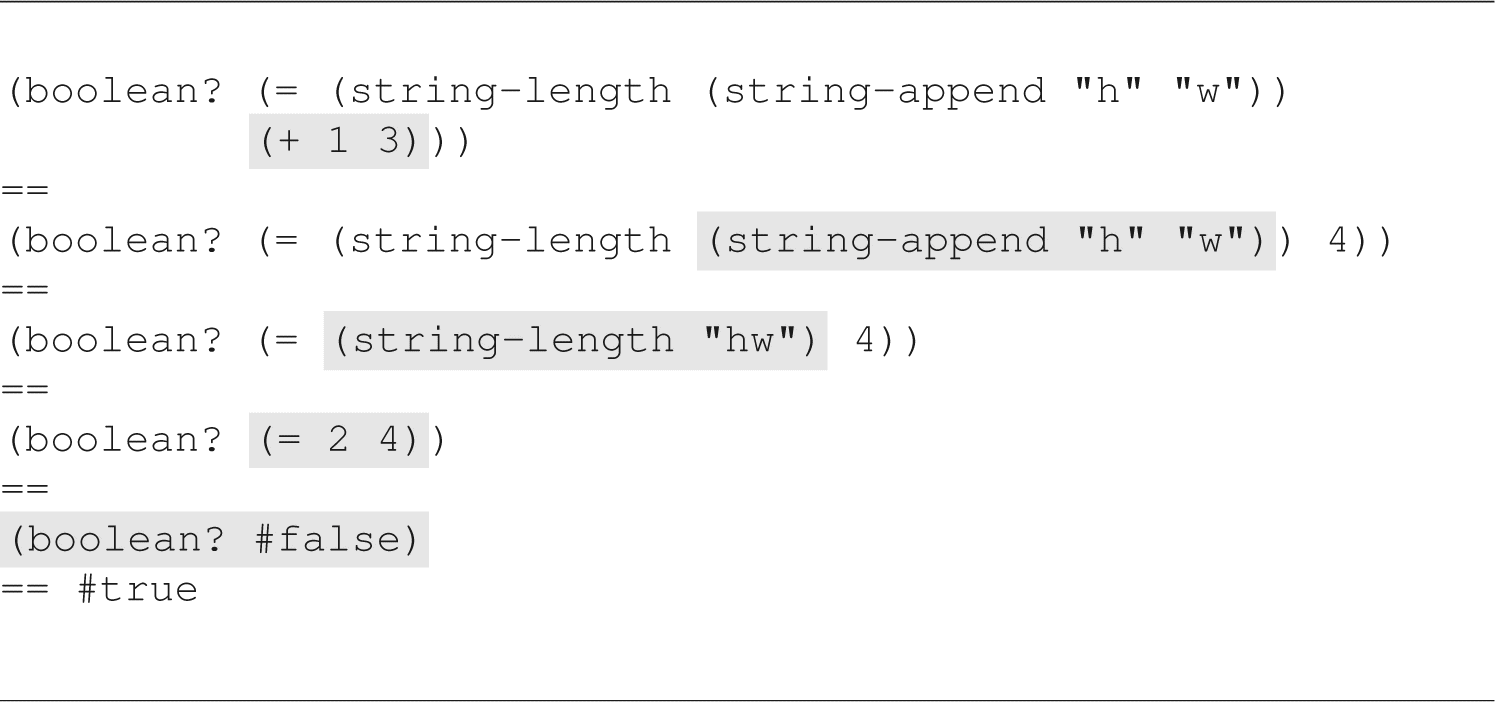
\includegraphics[width=0.85\textwidth]{images/00138.png}
  \caption{基于等量代换的算术归约示例}
  \label{fig:equals_by_equals}
\end{figure}

当对函数应用 \code{(f } $v_1 \dots v_n$\code{)} 求值时，只要所有实参 $v_i$ 都已经被计算为具体的值（Value），归约机制就会找到函数 \code{f} 的定义：
\begin{lstlisting}[language=BSL]
(define (f x_1 ... x_n) BodyExpression)
\end{lstlisting}
并将整个函数调用替换为 \code{BodyExpression}，其中所有的形参 $x_i$ 都被相应的实参值 $v_i$ 所替换！

\begin{exercise}{表达式单步归约推导}{121}
单步手工推演以下表达式的求值全过程：
\begin{lstlisting}[language=BSL]
(+ (* (/ 12 8) 2/3) (- 10 (sqrt 4)))
(cond [(= 0 0) #false] [(> 2 1) (string=? "a" "b")] [else (= 0 2)])
(cond [(= 2 0) #false] [(> 2 1) (string=? "a" "a")] [else (= 0 2)])
\end{lstlisting}
\end{exercise}

\begin{exercise}{函数调用单步推导}{122}
假设定义区包含以下定义：
\begin{lstlisting}[language=BSL]
(define (f x y)
  (+ (* 3 x) (* (+ y 1) 4)))
\end{lstlisting}
单步推演以下调用的计算过程：
\begin{lstlisting}[language=BSL]
(+ (f 1 2) (f 2 1))
(f 1 (* 2 3))
(f (f 1 (* 2 3)) 19)
\end{lstlisting}
\end{exercise}

% ==============================================================================
\intermezzosection{语义与计算 (Meaning and Computing)}
\label{sec:int01_computing}
% ==============================================================================

在 DrRacket 中，你无需仅凭纸笔进行上述推演。DrRacket 内置了世界一流的教学工具——\term{单步执行器}（The Stepper）。点击工具栏上的“Step”按钮，单步执行器将以绿色高亮当前正在被求值的子表达式（Redex），并以紫色高亮其代换后的结果。

每当你对某个复杂函数在特定输入下的执行路径感到困惑时，单步执行器就是你最权威、最直观的导师。

% ==============================================================================
\intermezzosection{BSL 错误 (BSL Errors)}
\label{sec:int01_errors}
% ==============================================================================

在编程中，错误主要分为两大范畴：
\begin{enumerate}
  \item \textbf{句法错误}（Syntax Errors）：代码不符合文法规则，程序根本无法被解析或启动；
  \item \textbf{运行时错误}（Runtime Errors）：代码符合文法，但在执行过程中遭遇了非法的算术或类型操作（如除以零、将数传递给需要字符串的函数等）。
\end{enumerate}

% ==============================================================================
\intermezzosection{布尔表达式 (Boolean Expressions)}
\label{sec:int01_boolean_expressions}
% ==============================================================================

逻辑运算 \code{and} 与 \code{or} 在 BSL 中具有特殊的“短路求值”（Short-Circuit Evaluation）语义：
\begin{itemize}
  \item \code{(and exp\_1 exp\_2 ...)}：从左到右求值。一旦某个表达式求得 \code{\#false}，整个 \code{and} 立即返回 \code{\#false}，后续表达式根本不会被计算！
  \item \code{(or exp\_1 exp\_2 ...)}：从左到右求值。一旦某个表达式求得 \code{\#true}，整个 \code{or} 立即返回 \code{\#true}，后续表达式被直接跳过。
\end{itemize}

事实上，\code{and} 与 \code{or} 本质上是 \code{cond} 表达式的语法糖：
\begin{align*}
\code{(and $e\_1$ $e\_2$)} &\equiv \code{(cond [$e\_1$ $e\_2$] [else \#false])} \\
\code{(or $e\_1$ $e\_2$)}  &\equiv \code{(cond [$e\_1$ \#true] [else $e\_2$])}
\end{align*}

\begin{exercise}{用 cond 重写 if 与 and}{123}
写出形式化规则，说明如何将任何形如 \code{(if condition then-exp else-exp)} 的表达式重构为等价的 \code{cond} 表达式。
\end{exercise}

% ==============================================================================
\intermezzosection{常量定义 (Constant Definitions)}
\label{sec:int01_constant_definitions}
% ==============================================================================

定义区的常量定义是自顶向下依次被求值的。一旦一个常量被绑定到值上，在该定义之后的任何地方都可以引用这个名字。

\begin{exercise}{常量定义的推导}{124}
单步推演以下程序的执行顺序，解释常量绑定与函数定义的依赖关系：
\begin{lstlisting}[language=BSL]
(define PRICE 5)
(define SALES-TAX (* 0.08 PRICE))
(define TOTAL (+ PRICE SALES-TAX))
\end{lstlisting}
\end{exercise}

% ==============================================================================
\intermezzosection{结构体类型定义 (Structure Type Definitions)}
\label{sec:int01_structure_type_definitions}
% ==============================================================================

结构体类型定义向语言中添加了构造函数、选择器与谓词。

特别需要明确：\textbf{结构体实例本身就是一种一等公民的“值”（Value）}。
例如，\code{(make-posn 3 4)} 是一个值；但 \code{(make-posn (+ 1 2) 4)} 并不是值，而是一个尚未完全求值的表达式，它需要先将各参数归约为值，才能生成最终的结构体实例。

\begin{exercise}{区分合法句子}{125}
甄别以下结构体相关语句的文法合法性：
\begin{lstlisting}[language=BSL]
(define-struct oops [])
(define-struct child [parents dob date])
(define-struct (child person) [dob extra])
\end{lstlisting}
\end{exercise}

\begin{exercise}{辨识结构体值}{126}
假设定义区包含 \code{(define-struct point [x y])}。在以下各项中，哪些已经是最终的“值”，哪些是仍需计算的表达式？
\begin{lstlisting}[language=BSL]
(make-point 1 2)
(make-point (make-point 1 2) 3)
(make-point (+ 1 2) 3)
\end{lstlisting}
\end{exercise}

\begin{exercise}{结构体字段提取推导}{127}
单步推导以下包含结构体选择器的复杂表达式：
\begin{lstlisting}[language=BSL]
(define-struct ball [x y deltax deltay])
(number? (ball-x (make-ball 1 2 3 4)))
(ball-deltax (make-ball 1 2 3 4))
\end{lstlisting}
\end{exercise}

% ==============================================================================
\intermezzosection{BSL 测试 (BSL Tests)}
\label{sec:int01_bsl_tests}
% ==============================================================================

测试是程序设计中不可或缺的基石。图~\ref{fig:bsl_full_grammar} 呈现了包含了完整测试机制的 BSL 终极文法。

\begin{figure}[htbp]
  \centering
  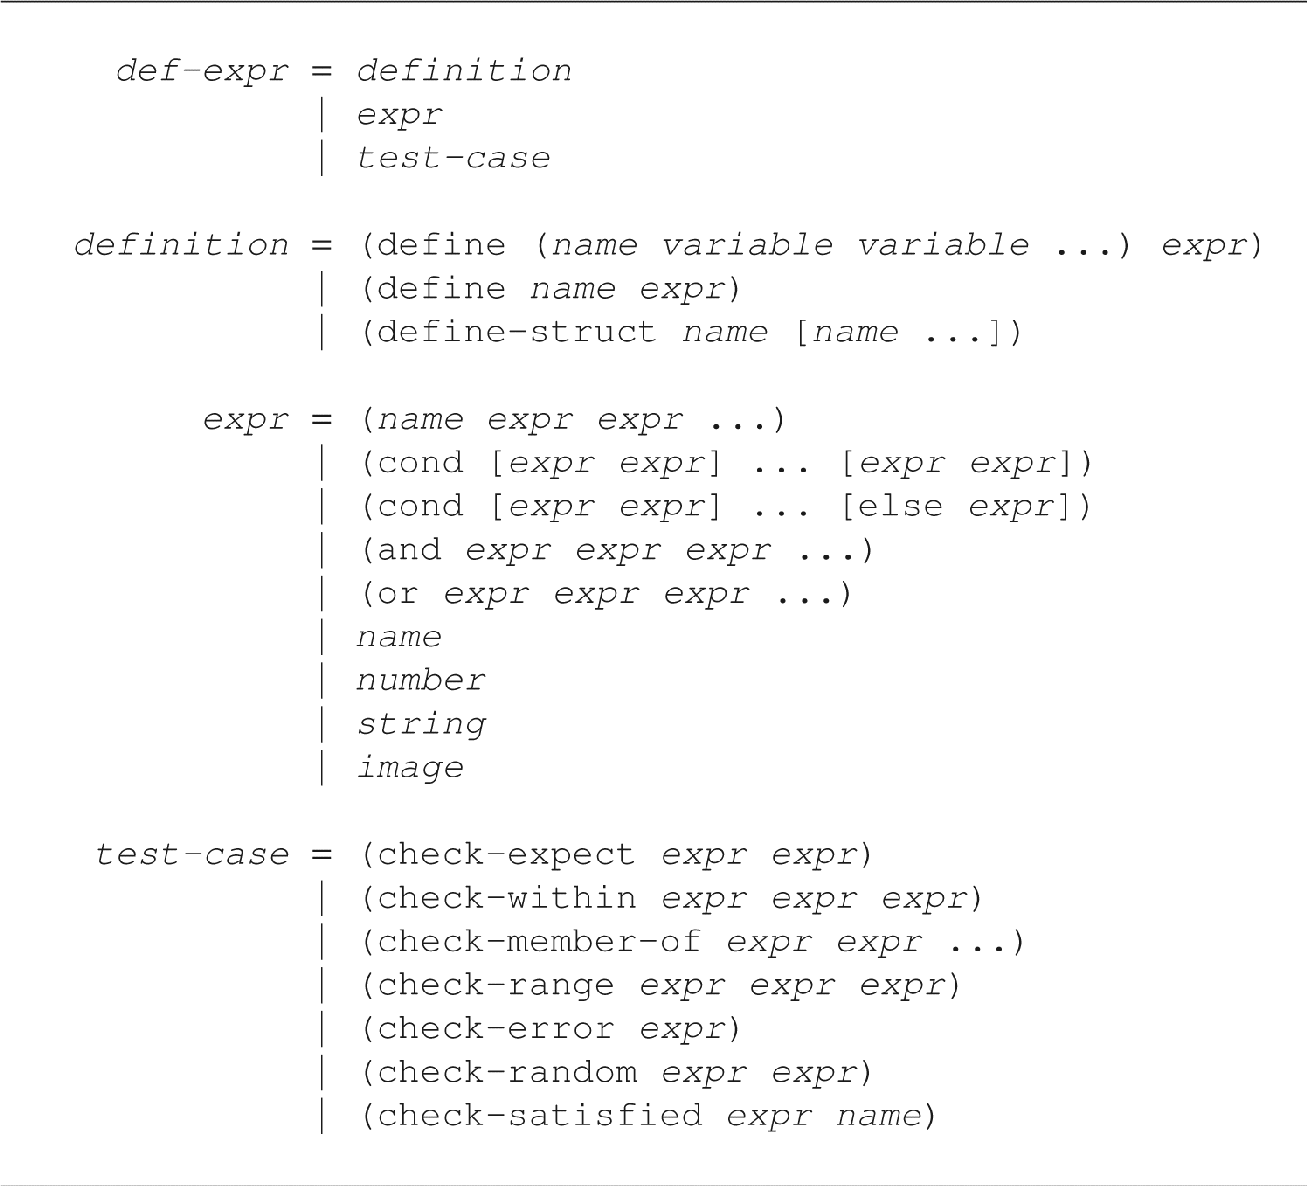
\includegraphics[width=0.85\textwidth]{images/00141.png}
  \caption{BSL 完整语法规范（包含测试套件）}
  \label{fig:bsl_full_grammar}
\end{figure}

BSL 提供了三种核心测试断言：
\begin{itemize}
  \item \code{(check-expect Expression\_1 Expression\_2)}：断言两个表达式产生严格完全相同的值；
  \item \code{(check-within Expression\_1 Expression\_2 Tolerance)}：用于浮点数或不精确数的近似比较（误差在 \code{Tolerance} 范围内）；
  \item \code{(check-error Expression ExpectedErrorMessage)}：断言前一个表达式必定抛出带有指定提示文本的运行时错误。
\end{itemize}

\begin{exercise}{运行单元测试套件}{128}
将以下测试复制到 DrRacket 定义区并运行，观察测试报告窗口的反馈：
\begin{lstlisting}[language=BSL]
(check-expect 3 3)
(check-member-of "green" "red" "yellow" "green")
(check-within (sqrt 2) 1.414 0.001)
(check-range 5 0 10)
(check-error (/ 1 0) "/: division by zero")
\end{lstlisting}
\end{exercise}

% ==============================================================================
\intermezzosection{BSL 错误信息详查 (BSL Error Messages)}
\label{sec:int01_error_messages}
% ==============================================================================

面对错误提示时的沉着与从容，是新手迈向专业程序员的重要标志。下文汇总了初学者在 BSL 中最常遭遇的典型错误场景。

\subsection{函数应用相关错误}

假设定义区仅有 \code{(define (average x y) (/ (+ x y) 2))}。

\begin{figure}[htbp]
  \centering
  
\includegraphics[width=0.75\textwidth]{images/00145.png}
  \caption{未定义函数错误：调用了不存在的函数名}
  \label{fig:err_undefined_fn}
\end{figure}

\begin{figure}[htbp]
  \centering
  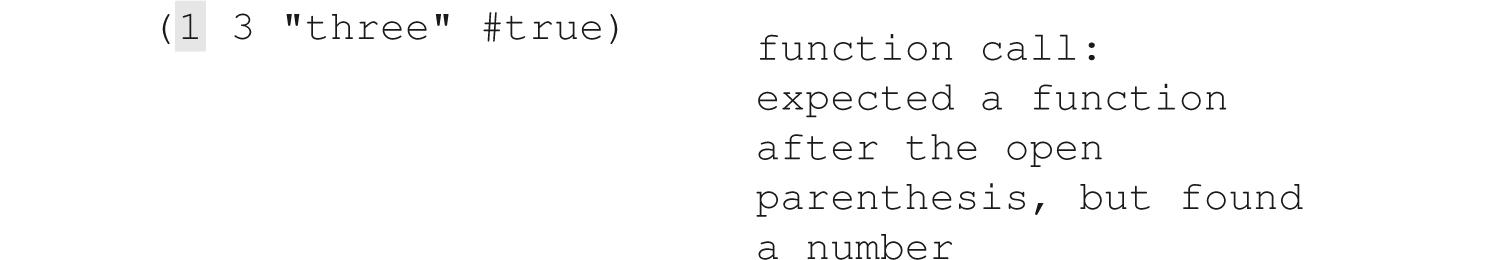
\includegraphics[width=0.75\textwidth]{images/00146.png}
  \caption{括号后缺少函数名：开括号后紧跟了数值而不是操作符}
  \label{fig:err_expected_fn}
\end{figure}

\begin{figure}[htbp]
  \centering
  
\includegraphics[width=0.75\textwidth]{images/00147.png}\\[1ex]
  
\includegraphics[width=0.75\textwidth]{images/00148.png}
  \caption{实参个数不匹配：传入参数过少（上）或过多（下）}
  \label{fig:err_arg_mismatch}
\end{figure}

\subsection{数据类型不匹配错误}

\begin{figure}[htbp]
  \centering
  
\includegraphics[width=0.75\textwidth]{images/00150.png}\\[1ex]
  
\includegraphics[width=0.75\textwidth]{images/00151.png}
  \caption{类型契约违背：向选择器或算术操作符传递了错误类型的值}
  \label{fig:err_type_contract}
\end{figure}

如图~\ref{fig:err_type_contract} 所示，\code{posn-x} 期望接收一个 \code{posn} 结构体，却收到了整数 73；算术加法 \code{+} 期望接收数值，却收到了字符串 \code{"hello"}。

\subsection{条件表达式与定义相关错误}

\begin{figure}[htbp]
  \centering
  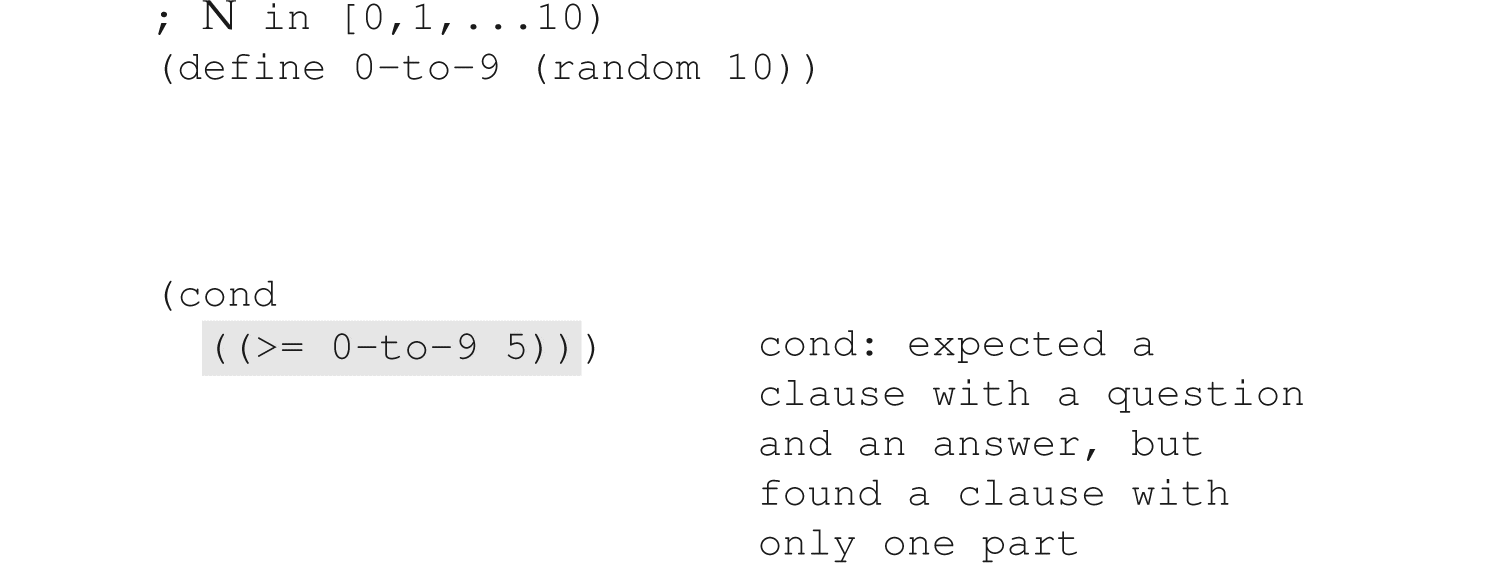
\includegraphics[width=0.75\textwidth]{images/00152.png}\\[1ex]
  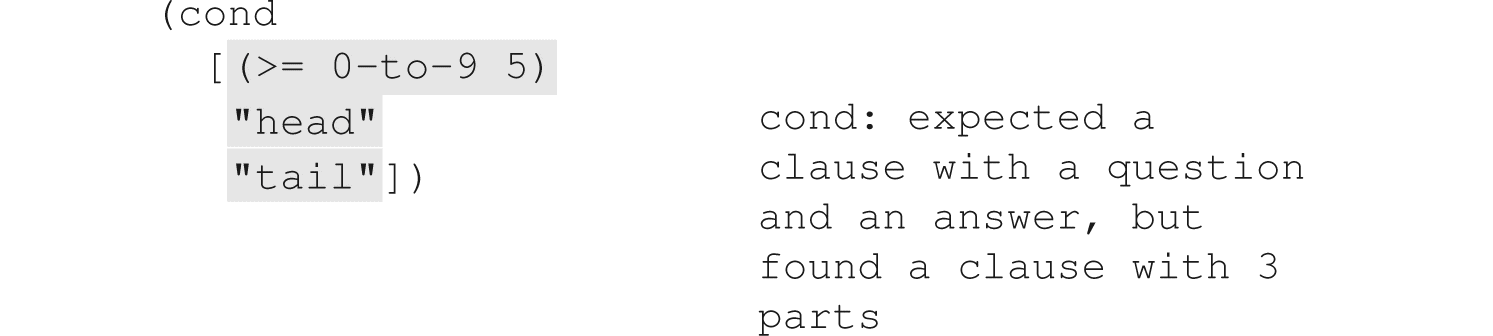
\includegraphics[width=0.75\textwidth]{images/00153.png}
  \caption{cond 分支格式错误}
  \label{fig:err_cond_shape}
\end{figure}

\begin{figure}[htbp]
  \centering
  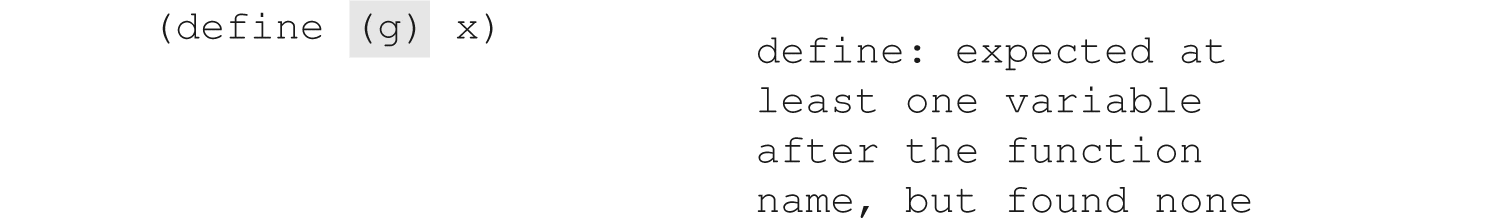
\includegraphics[width=0.75\textwidth]{images/00157.png}\\[1ex]
  
\includegraphics[width=0.75\textwidth]{images/00158.png}
  \caption{函数头缺少参数或语法格式错误}
  \label{fig:err_redefinition}
\end{figure}

当你在编写代码遭遇错误时，请沉着阅读高亮提示并对照上述图集，追溯文法与类型规范，你将能够迅速定位根因并优雅修正！
